% Appendix Template
\chapter{Mass Spectrometry} % Main appendix title
\label{AppendixB} % Change X to a consecutive letter; for referencing this appendix elsewhere, use \ref{AppendixX}

\begin{figure}[ht!]
\centering
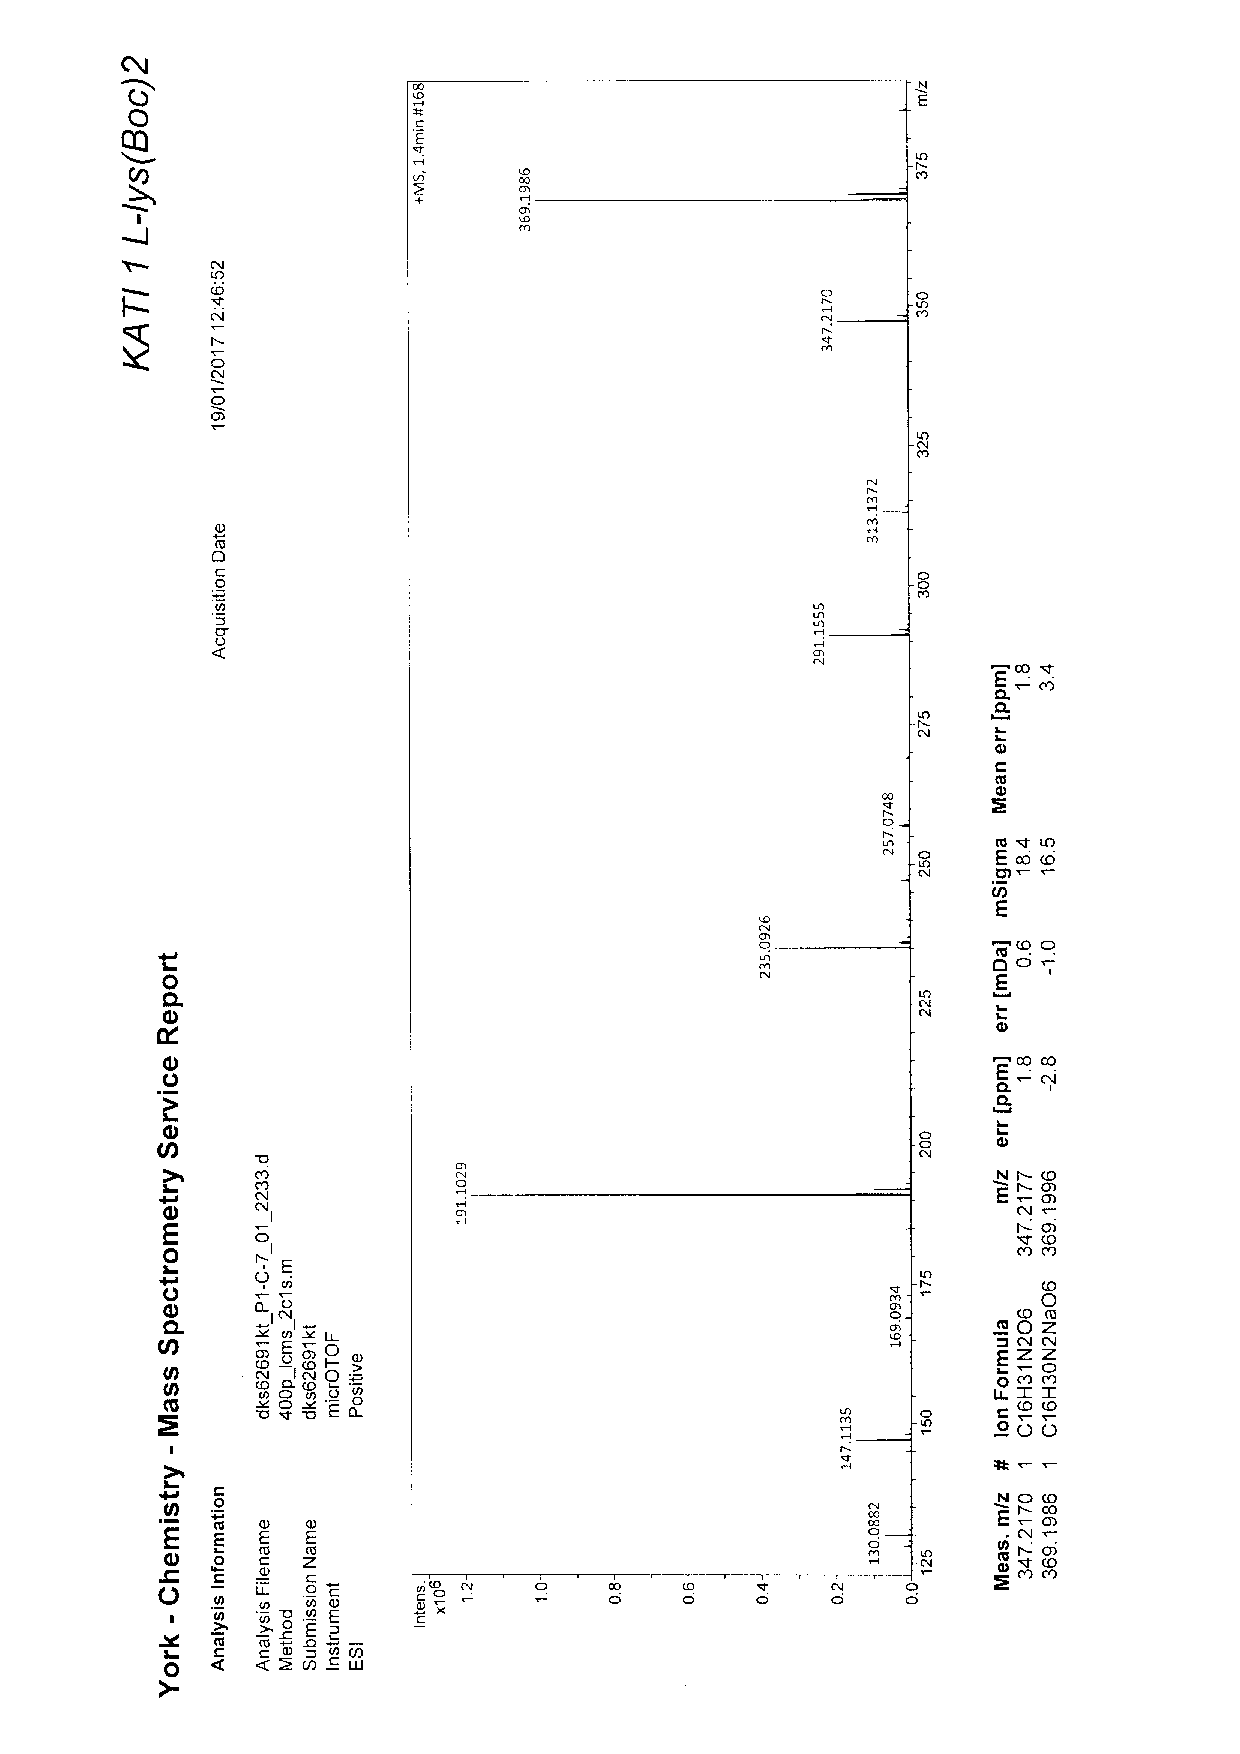
\includegraphics[scale=0.75]{Mass_Spec/KAT1_1.PDF}
\caption{Mass Spectrometry analysis of L-Lysine(Boc)\textsubscript{2}}
\end{figure}

\begin{figure}[ht!]
\centering
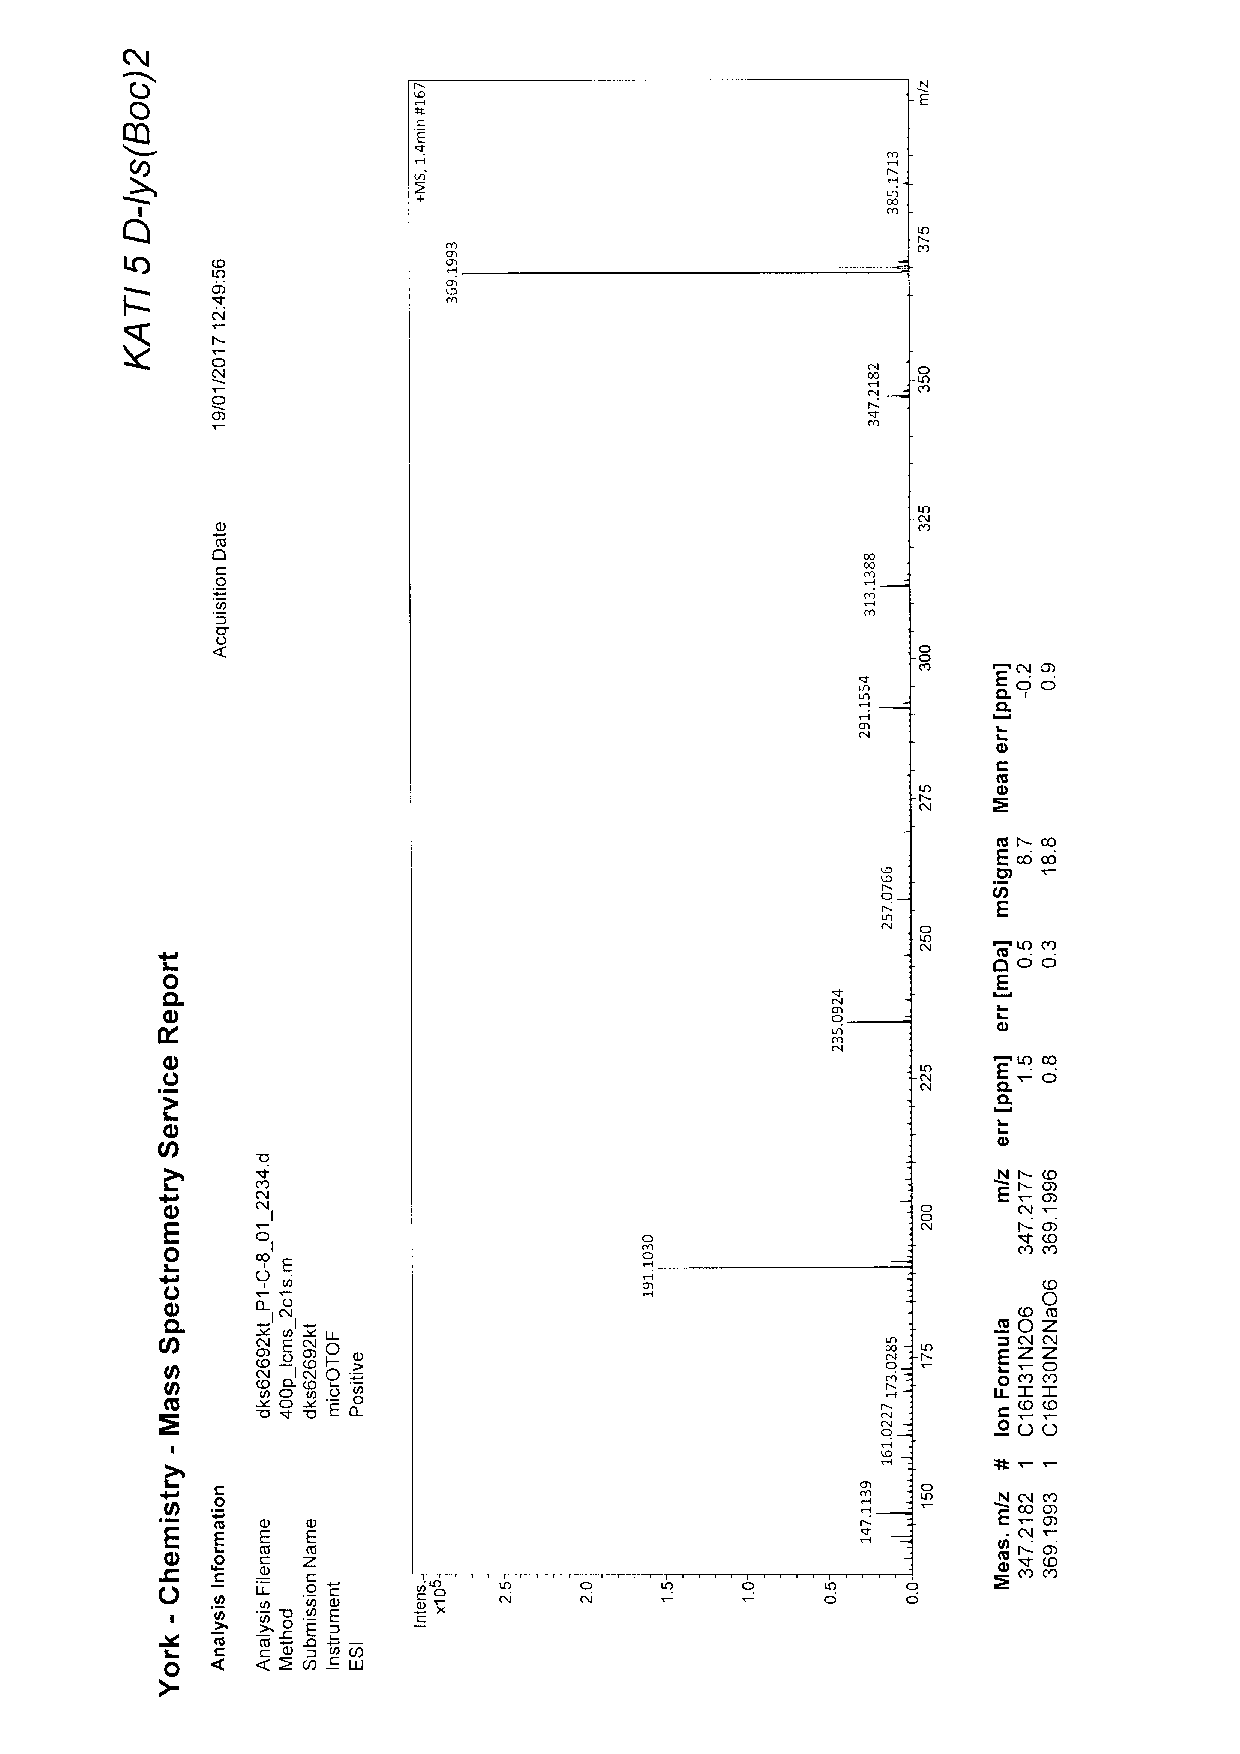
\includegraphics[scale=0.75]{Mass_Spec/KAT1_5.PDF}
\caption{Mass Spectrometry analysis of D-Lysine(Boc)\textsubscript{2}}
\end{figure}

\begin{figure}[ht!]
\centering
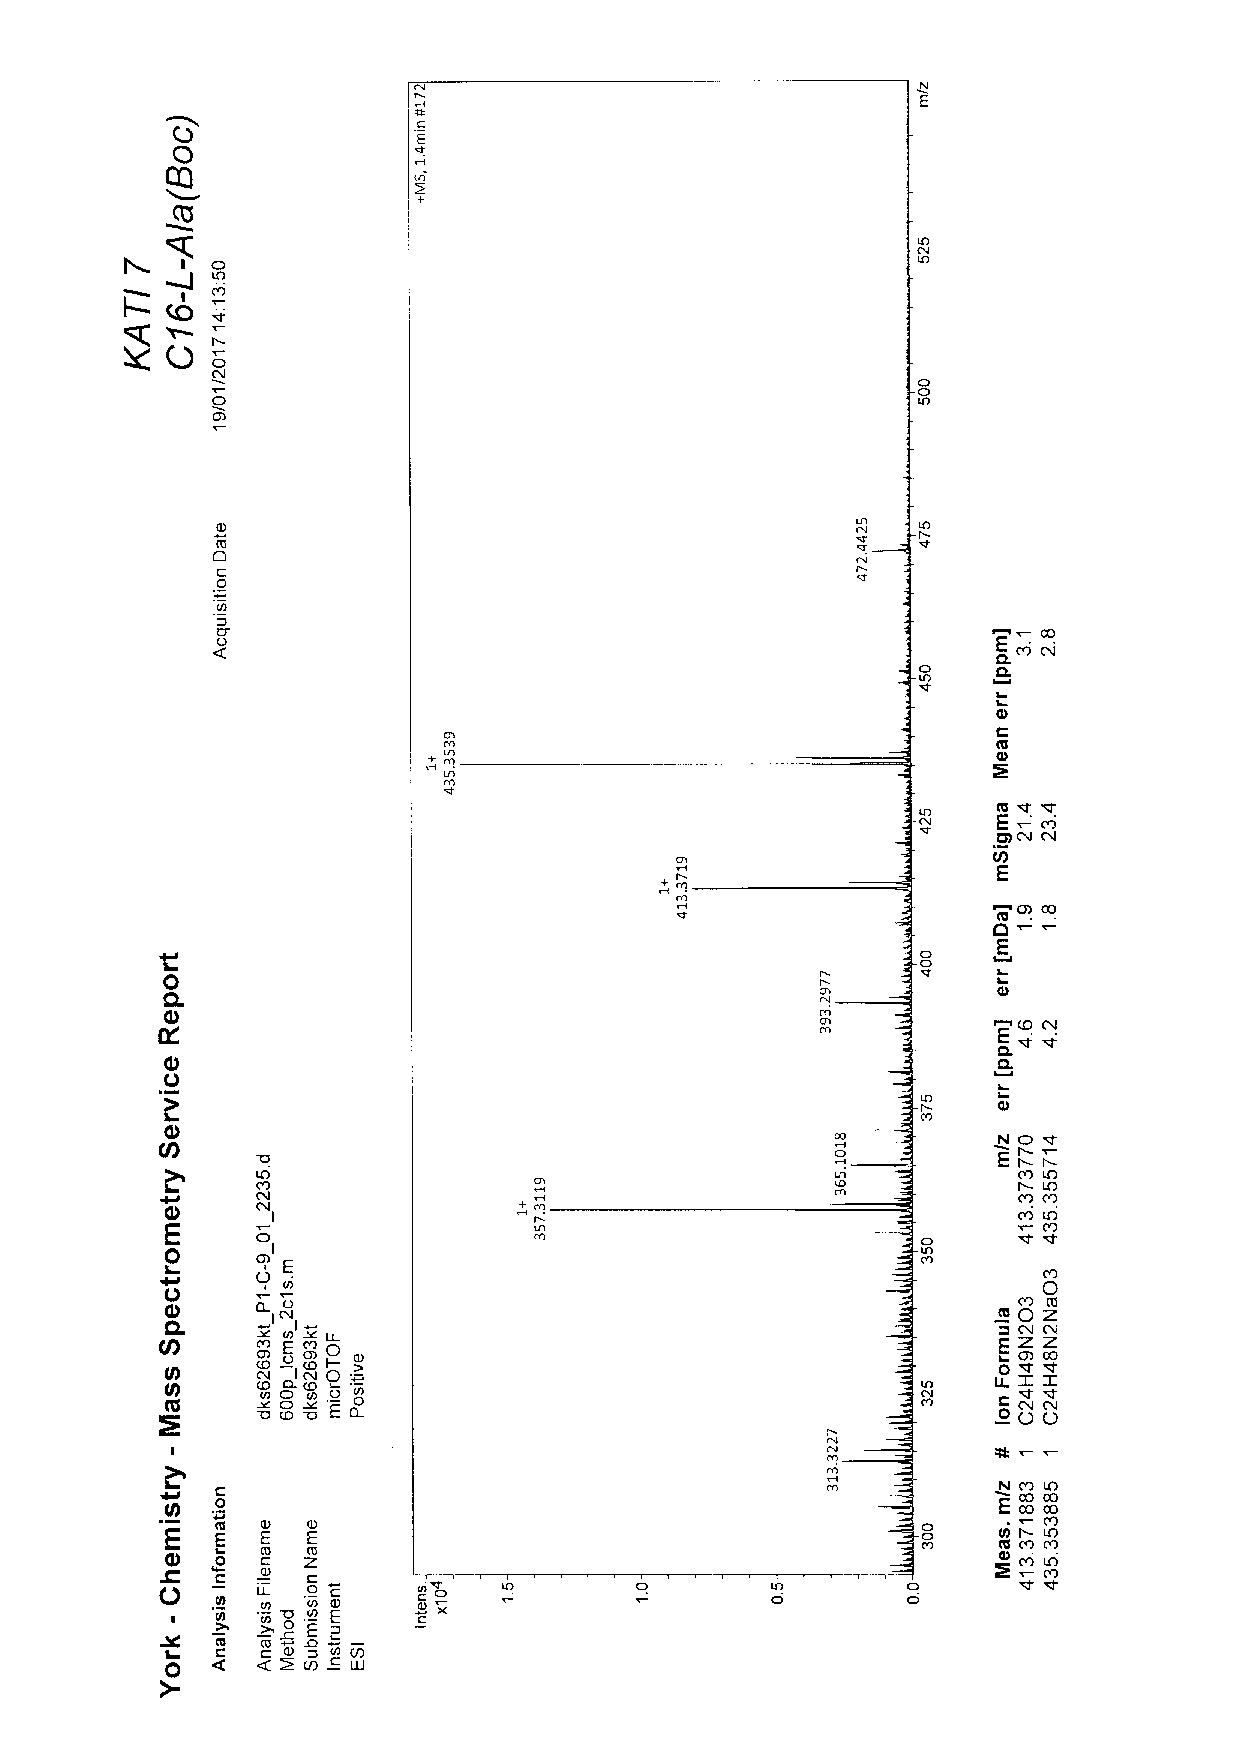
\includegraphics[scale=0.75]{Mass_Spec/KAT1_7.PDF}
\caption{Mass Spectrometry analysis of C16-L-Ala(Boc)}
\end{figure}

\begin{figure}[ht!]
\centering
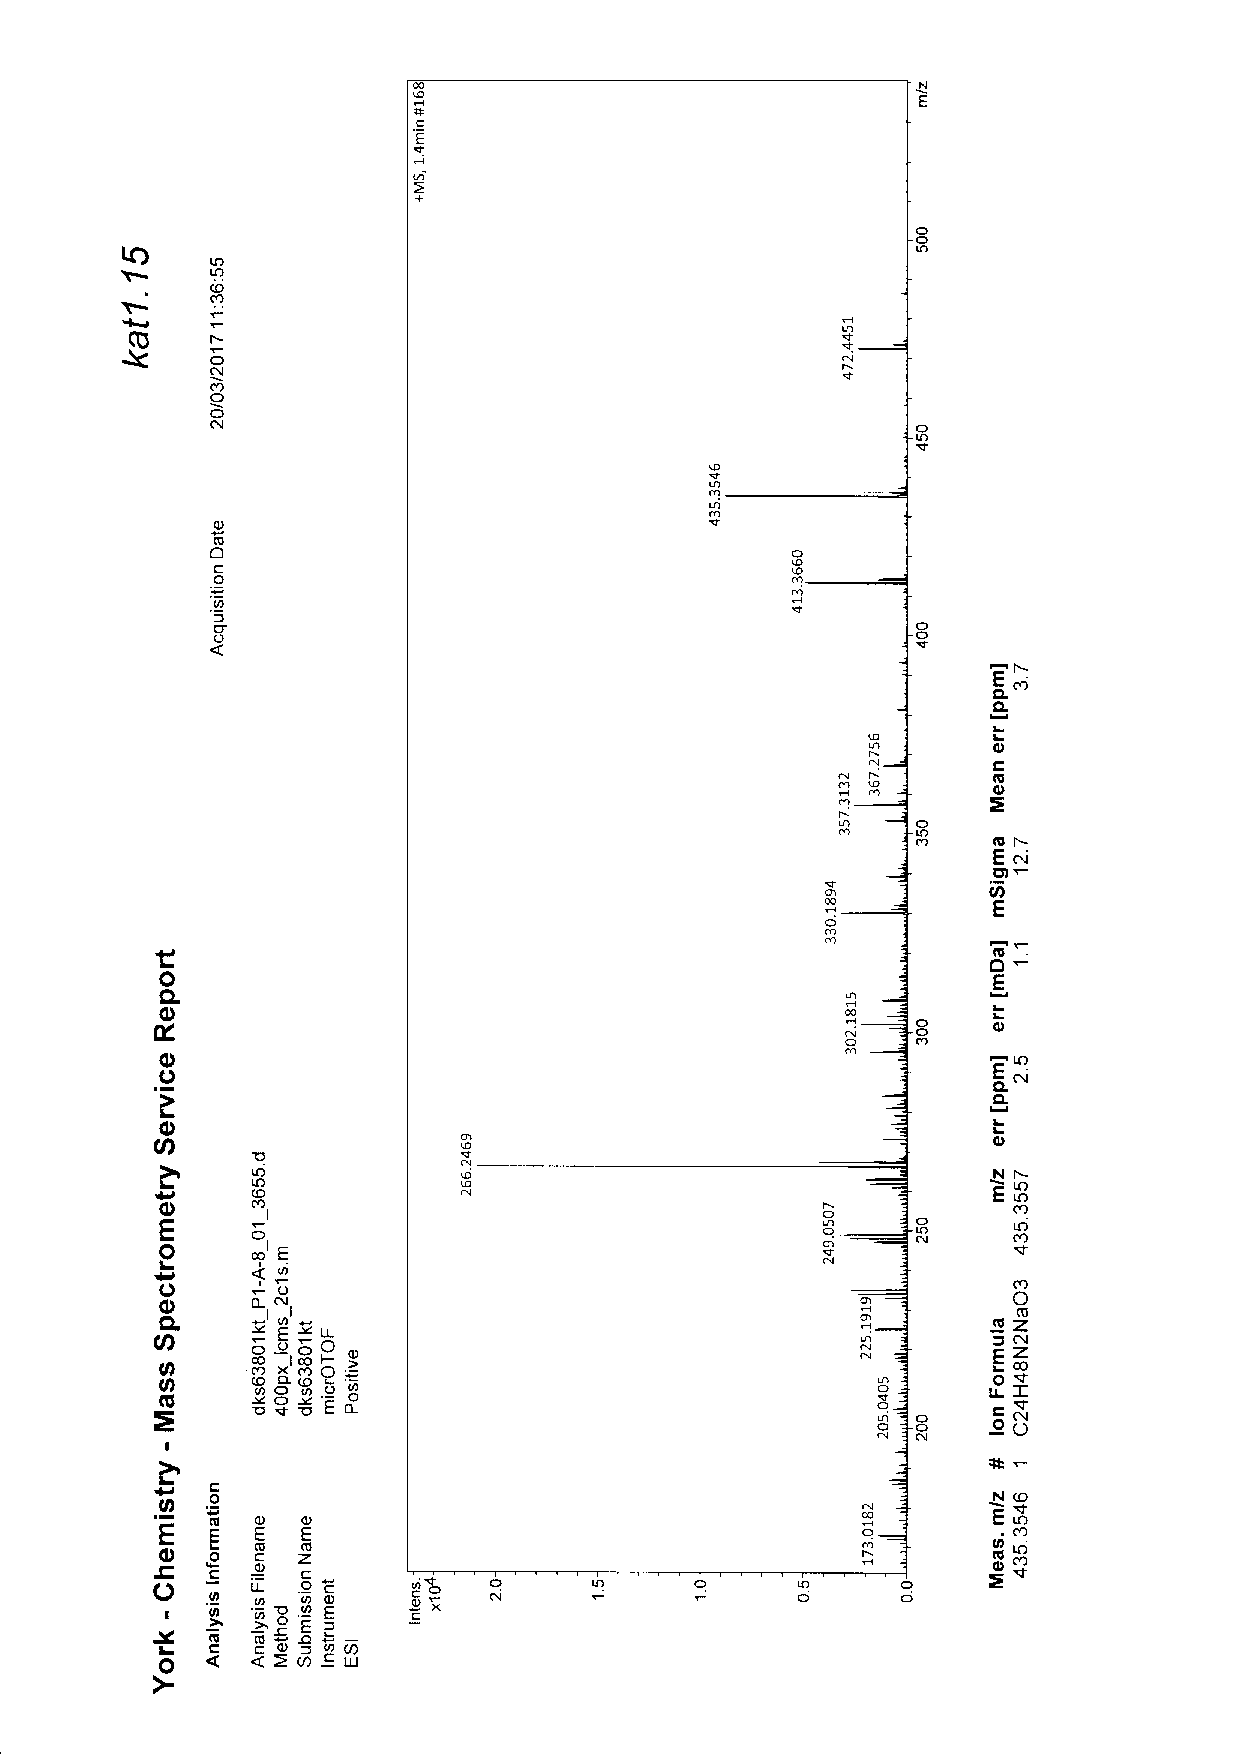
\includegraphics[scale=0.75]{Mass_Spec/KAT1_15.PDF}
\caption{Mass Spectrometry analysis of C16-D-Ala(Boc)}
\end{figure}

\begin{figure}[ht!]
\centering
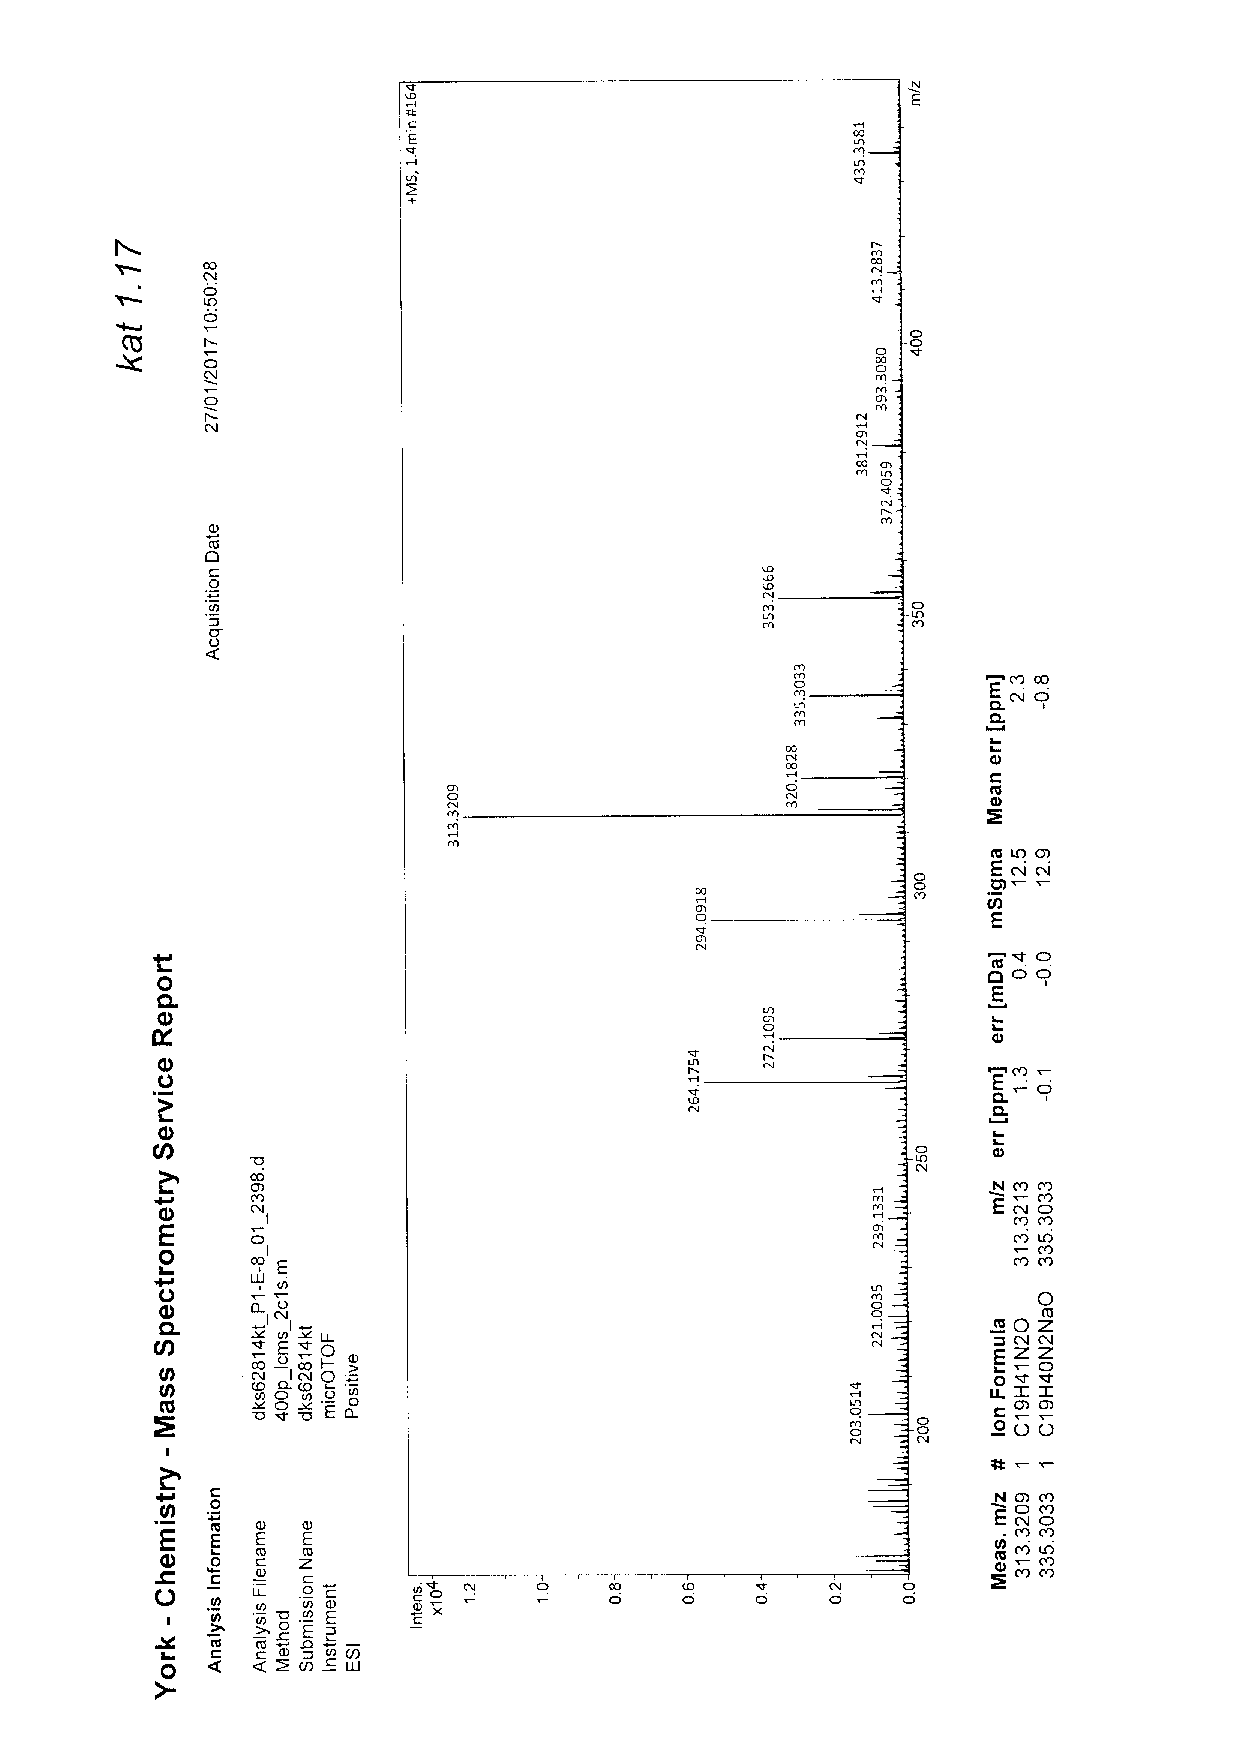
\includegraphics[scale=0.75]{Mass_Spec/KAT1_17.PDF}
\caption{Mass Spectrometry analysis of C16-L-Ala}
\end{figure}

\begin{figure}[ht!]
\centering
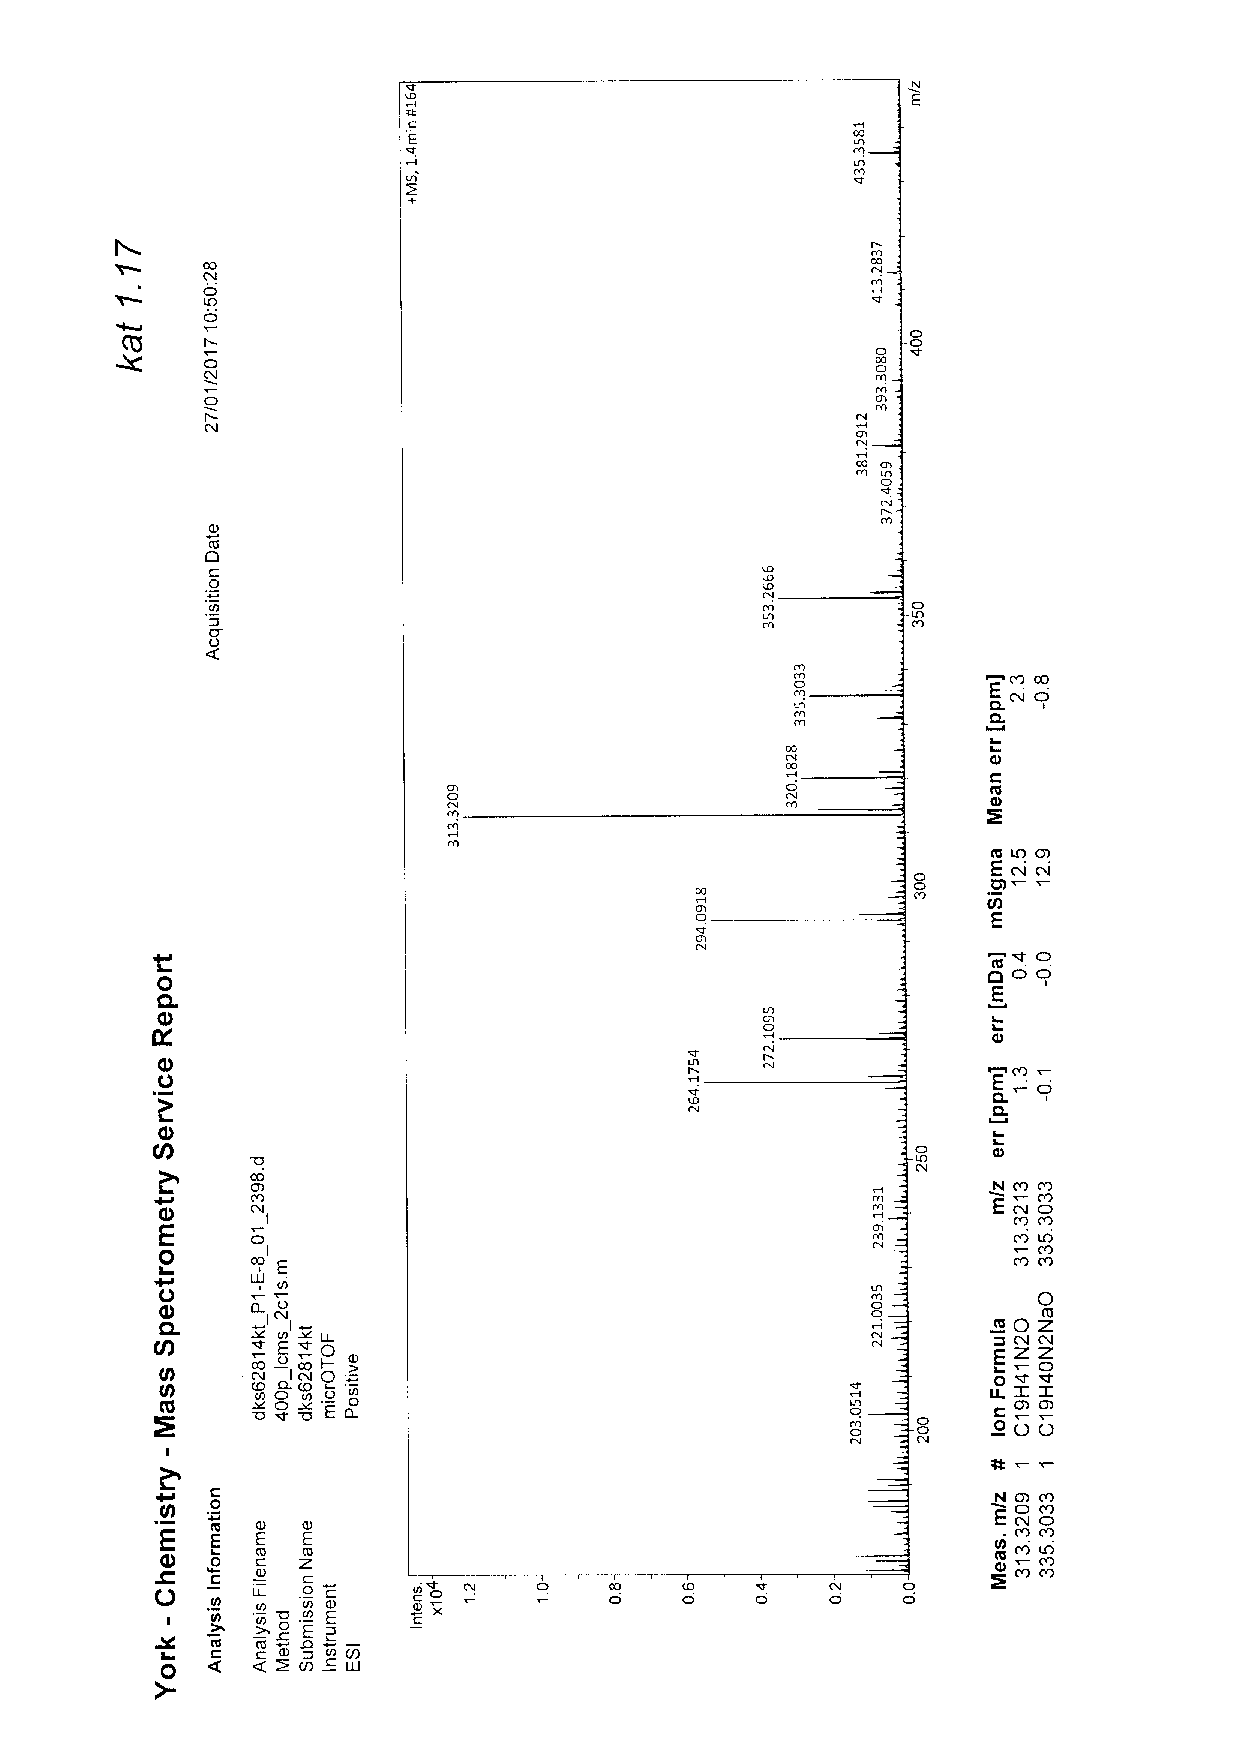
\includegraphics[scale=0.75]{Mass_Spec/KAT1_17.PDF}
\caption{Mass Spectrometry analysis of C16-D-Ala}
\end{figure}

\begin{figure}[ht!]
\centering
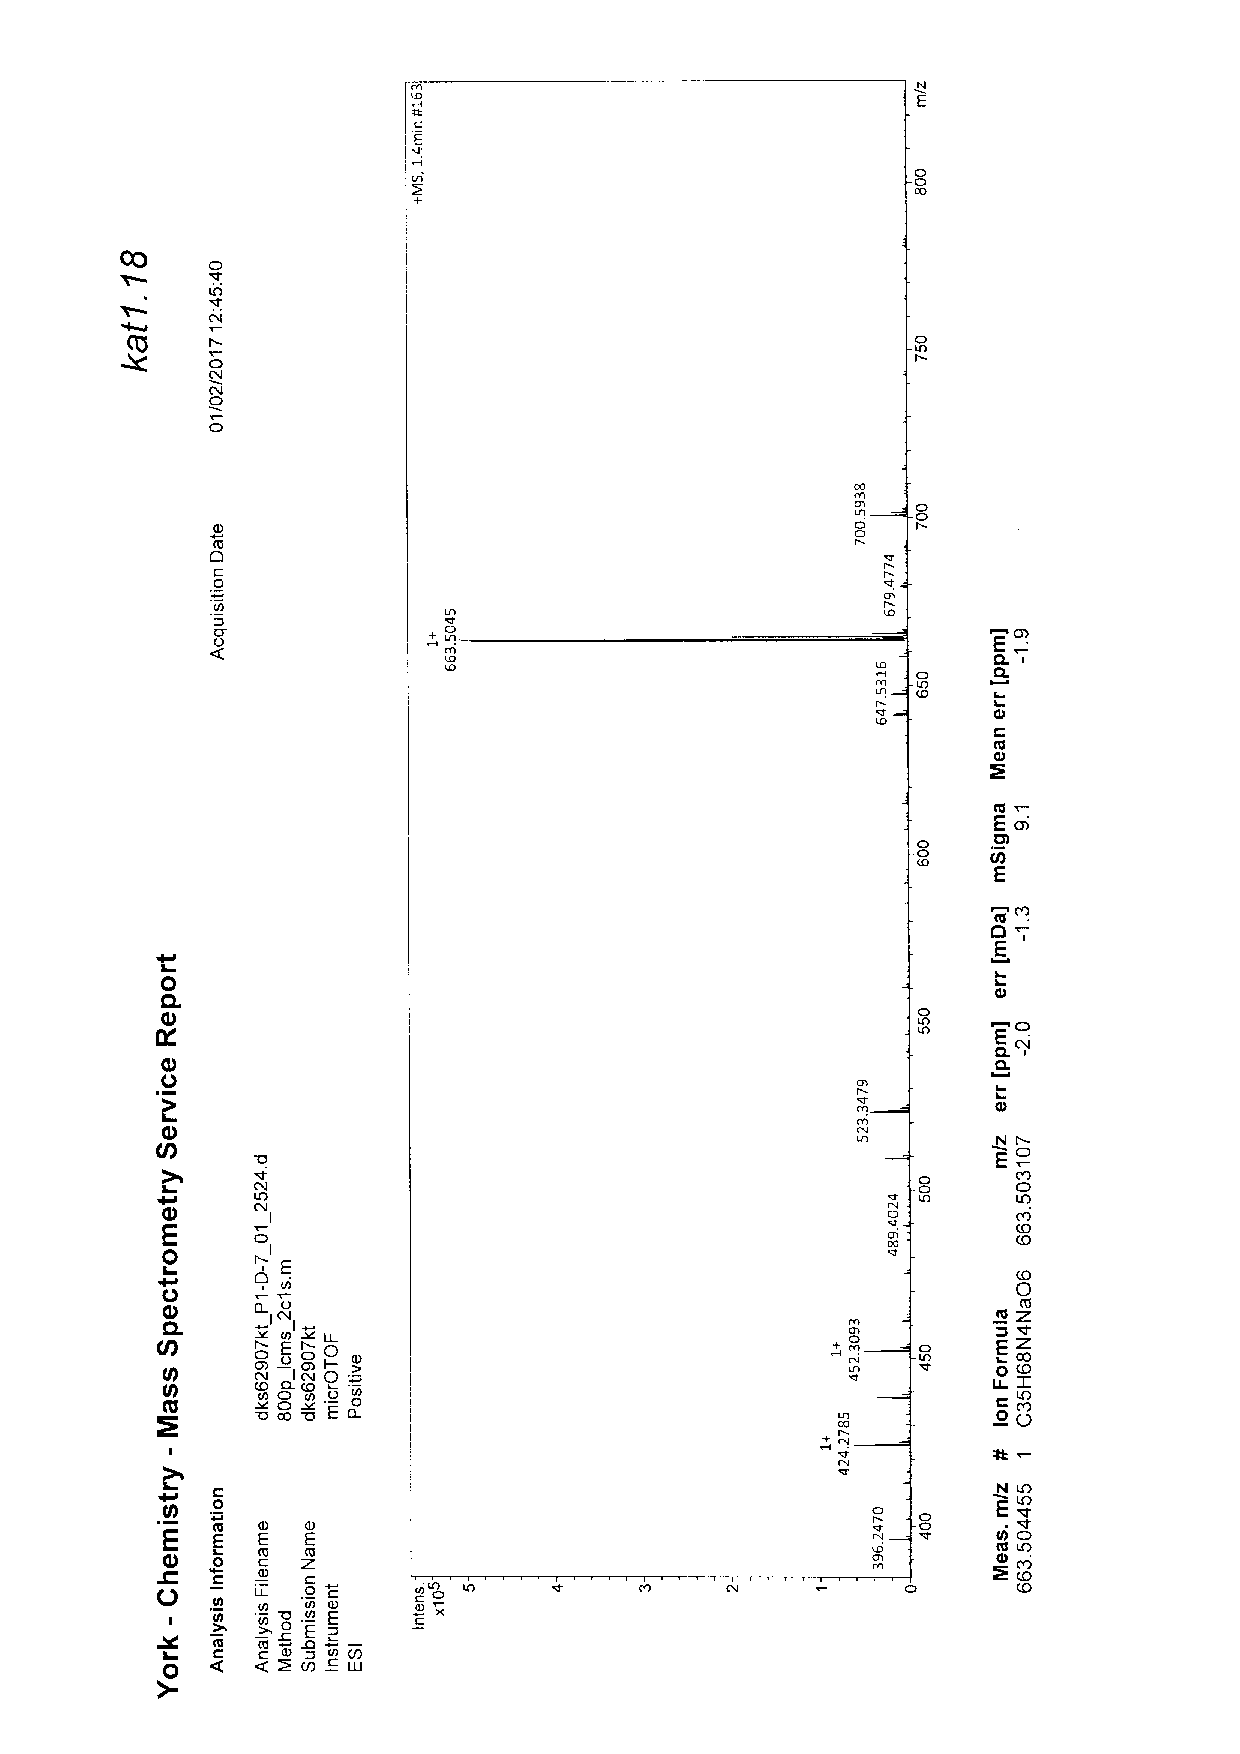
\includegraphics[scale=0.75]{Mass_Spec/KAT1_18.PDF}
\caption{Mass Spectrometry analysis of C16-L-Ala-L-Lys(Boc)\textsubscript{2}}
\end{figure}

\begin{figure}[ht!]
\centering
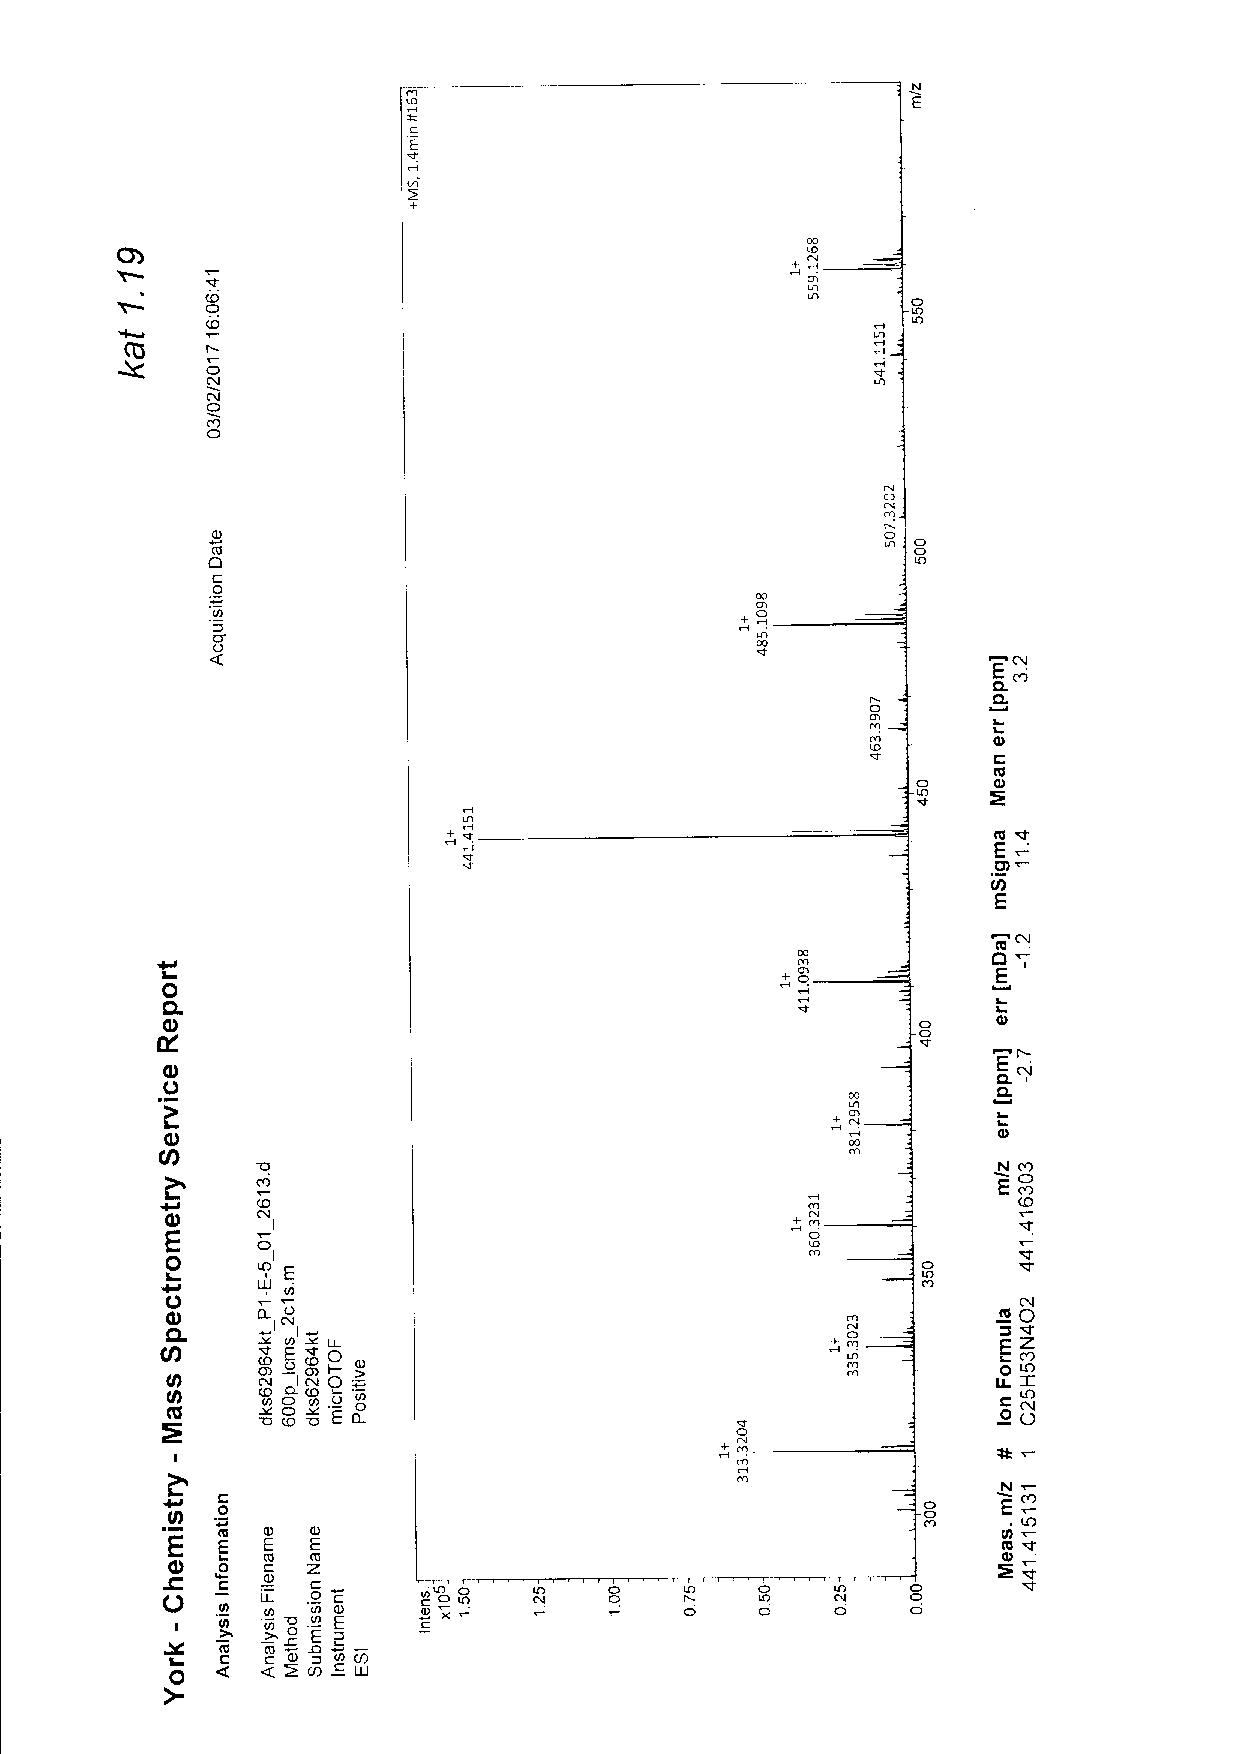
\includegraphics[scale=0.75]{Mass_Spec/KAT1_19.PDF}
\caption{Mass Spectrometry analysis of C16-L-Ala-L-Lys}
\end{figure}
